%!TEX root = TIHSC_Project_main.tex
\chapter{Introduction}
The problem stated in this project is ``doing texton mapping quicker''.
Texton mapping is an algorithmic tool to make intelligent edge detection on images. 
When a human looks at an image the ability to draw edges around objects is very easy, 
especially when the objects are well-known for the human. 
Comuputers do not have that ability because edge detection typically depends on gradient filtering.

\begin{figure}[H]
\centering
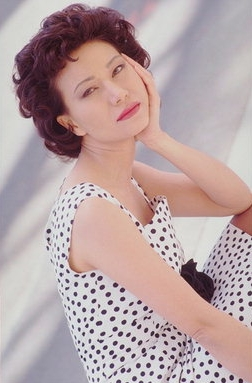
\includegraphics[width = 0.5\linewidth]{prikpige}
\caption{Original picture}
\label{fig:prikpige}
\end{figure}

The image in figure \ref{fig:prikpige} shows a girl in a dotted dress. 
For the human eye it is easy to distinguish between dress and skin. 
Normal edge detection will not be able to do this distinction, 
on the contrary emphasize all the textures in the dress too.

\section{Texton filtering}
\label{sec:TextonFiltering}
By filtering an image with several filters emphasizing dots and lines at different sizes and angels, 
one can achieve a feature vector for every pixel. 
The feature vector has a size of $<N\_PIXELS\times DIMENSIONS>$ and is collapsed into a single column vector. 

%BILLEDE AF DE FEMTEN FILTRE
\begin{figure}[H]
\centering
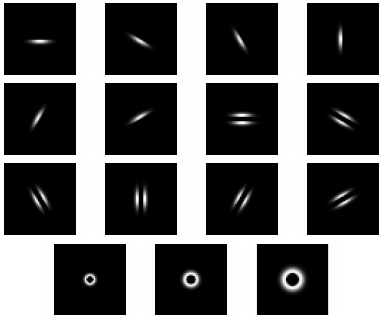
\includegraphics[width = 0.707\linewidth]{filters}
\caption{The 15 filters (49 x 49 pixels)}
\label{fig:filtre}
\end{figure}


This feature vector contains information about the pixel's belonging to a certain texture. 
After filtering an image with one filter the result is a new image where every pixel has a new value. 
This value correspond to one of the dimensions in the feature vector, which has 15 dimensions.

To find out where the textures are a classification of the feature vectors is needed. 
For the texton mapping k-means clustering is ideal for this classification.


\subsection{K-means}
\label{sec:Kmeans}
K-means clustering is an unsupervised classification and takes an n-dimensional feature vector and splits it into $C$ clusters. 
In this case the 15 filters makes a 15-dimensional feature vector and it is split into 64 clusters. 

To make the classification 64 random points are picked among the existing features, this is now the centers of the clusters. 
Then the distance from every feature (1 pixel represented by the 15-dimensional feature vector) to the center is calculated. 
Now the pixel is assigned to the closest center and now belongs to that cluster. 
The distance is calculated by euclidean distance, see equation \ref{eq:distance}.

\begin{equation}
\label{eq:distance}
d_p = \sqrt{(c-f_p)^2},
\end{equation}

where $c$ is the center and $f_p$ is a feature point, both in 15 dimensions. The distance, $d_p$, is a scalar.

After calculating all the distances a new center is calculated. 
This is done by calculating the mean value of the assigned points, see equation \ref{eq:meanvalue}.

\begin{equation}
\label{eq:meanvalue}
\mu_C = \frac{1}{|C_k|}\sum_{f\in C_k}f,
\end{equation}

where $\mu_C$ is the new center of cluster $C$ and $f$ is the points in cluster $C$.

These two steps are repeated for a number of iteration or until the center move less than a stated limit. 
In this project the number of iterations are fixed to 1000 and no limit is put into the movement of the centers.

When the k-means classification is done every pixel belongs to one of the 64 clusters. 
The result (a vector with N\_PIXELS indexes) can be 
converted to a matrix with the dimensions of the 
original image and plotted in Matlab.

\begin{figure}[H]
\centering
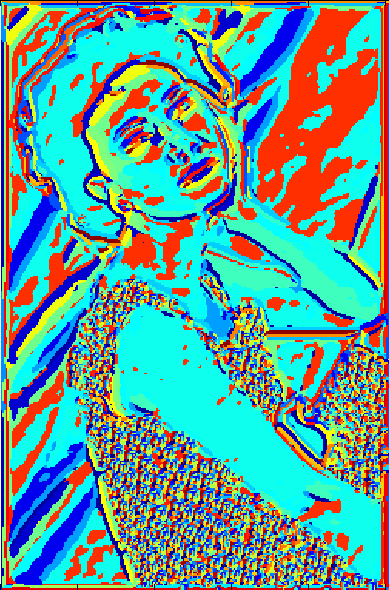
\includegraphics[width = 0.5\linewidth]{result_image}
\caption{The texton map of the original image}
\label{fig:result}
\end{figure}



\section{Execution time}
The texton filtering has been implemented on a CPU and run with 1000 iterations of k-means. 
The execution time for this operation was about 1200 seconds (20 min.) 
Acceleration via hardware implementation is expected to get the execution time down to 1 minute. 
Measurements for the different parts of the algorithm shows that the distance calculation in the k-means has a very long duration every iteration. 
Therefore focus is on this part.

